\documentclass[11pt]{article}

\usepackage[centering,top=1.5in,bottom=1.2in,left=1.4in,right=1.4in]{geometry}
\usepackage{amsmath,amssymb,mathtools}
\usepackage{booktabs}
\usepackage{graphicx}
\usepackage{float}
\usepackage{hyperref}
\usepackage{microtype}
\emergencystretch=3em

\title{Monte Carlo Counterfactual Regret Minimization}
\author{}
\date{\today}

\begin{document}

\maketitle

\begin{abstract}
This report studies Monte Carlo Counterfactual Regret Minimization
(MCCFR), focusing on the external-sampling variant. The project builds on
a previous implementation of full-tree CFR for Kuhn Poker and asks what
changes when the regret update is estimated from sampled trajectories
instead of a complete traversal of the game tree. I implement both
full-tree CFR and external-sampling MCCFR in Python, compare them on Kuhn
Poker, and use exact best responses to measure exploitability. The main
message is that MCCFR keeps the same local regret-minimization structure
as CFR, but replaces exact counterfactual values with sampled estimates.
\end{abstract}

\section{From CFR to MCCFR}

Counterfactual Regret Minimization (CFR) is a regret-minimization method
for extensive-form games with imperfect information. The key idea is to
place a small regret minimizer at every information set. At each iteration,
the algorithm computes a counterfactual value for every legal action at
each information set, updates local regrets, and then obtains the next
behavioral strategy by regret matching.

In the full-tree version of CFR, the update is exact for the current
strategy profile because it traverses the entire game tree. This is very
clear pedagogically, but it is also the bottleneck: one iteration costs
time proportional to the size of the tree. Kuhn Poker is tiny, so this is
not an issue there. In larger games such as poker variants with more
cards, betting actions, or public states, a full traversal can become too
expensive.

MCCFR keeps the same local regret-minimization structure but estimates
the counterfactual update by sampling part of the tree. The version
studied here is \emph{external sampling}. When updating player $i$, chance
nodes and opponent nodes are sampled, while player $i$'s own decision
nodes branch over all legal actions. Therefore, when the sampled path
reaches an information set of player $i$, the algorithm can still compare
all actions at that information set:
\[
R_i^T(I,a)
\leftarrow
R_i^{T-1}(I,a)
+ \widehat v_i(I,a) - \widehat v_i(I),
\]
where the hats indicate sampled estimates. The important point is that
this has the same form as the CFR regret update, but the values are
computed using a sampled subtree instead of the whole tree.

\section{Kuhn Poker as the Test Game}

Kuhn Poker is a small two-player zero-sum poker game introduced by Kuhn
\cite{kuhn1950}. The deck contains three cards, usually denoted
$J,Q,K$. Each player antes one chip and receives one private card. Player
0 acts first and can either check or bet. If player 0 checks, player 1 can
check or bet. If a bet occurs, the other player can call or fold. If no
one folds, the higher card wins the pot.

The game is small enough that every strategy and best response can be
computed exactly, but it still contains the main modeling features that
make poker interesting:
\begin{itemize}
\item private information, because each player only observes their own
card;
\item sequential decisions, because betting history affects later actions;
\item information sets, because the same private card and public history
can arise under different hidden opponent cards;
\item bluffing, because weak hands sometimes bet in equilibrium.
\end{itemize}

The known value of Kuhn Poker for player 0 is
\[
v^\star = -\frac{1}{18} \approx -0.055556.
\]
This value is useful as a sanity check: if an implementation converges to
a strategy profile whose expected payoff is far from this value, then
something is probably wrong.

In the code, the game is represented as a simple dictionary of nodes. A
chance node stores the six equally likely deals:
\[
KQ, QK, JK, KJ, QJ, JQ.
\]
A decision node stores the acting player, the information set, and the
legal actions. A terminal node stores the zero-sum utility vector. This is
not intended to be a general game engine. The point is to make the
algorithm readable and to keep the representation close to the game tree.

\section{Regret Matching and Full-Tree CFR}

Regret matching is the local learning rule used in this project. Suppose
an information set has action set $A$. Let $R^T(a)$ be the cumulative
regret for action $a$ after $T$ updates. Regret matching chooses the next
mixed action by normalizing only the positive regrets:
\[
\sigma^{T+1}(a)
=
\begin{cases}
\dfrac{[R^T(a)]_+}{\sum_{b \in A}[R^T(b)]_+},
& \text{if } \sum_{b \in A}[R^T(b)]_+ > 0, \\[1.2ex]
\dfrac{1}{|A|},
& \text{otherwise}.
\end{cases}
\]
The uniform fallback matters early in training because all regrets start
at zero.

In full-tree CFR, each information set has its own regret table. At each
iteration and for each update player $i$, the algorithm recursively
traverses the full game tree. Let $I$ be an information set of player
$i$, and let $a \in A(I)$. The update has the form
\[
R_i^T(I,a)
\leftarrow
R_i^{T-1}(I,a)
+ \pi_{-i}^{\sigma^T}(I)
\left(v_i(\sigma^T_{I \to a}, I) - v_i(\sigma^T, I)\right).
\]
Here $\pi_{-i}^{\sigma^T}(I)$ is the counterfactual reach probability
from chance and the opponent, $v_i(\sigma^T_{I \to a}, I)$ is the
counterfactual value of deviating to action $a$ at $I$, and
$v_i(\sigma^T, I)$ is the value of following the current mixed action at
$I$.

For implementation, this can be written more concretely. At an update
player node, recursively compute one child value for each legal action:
\[
u(a) = \text{value returned by the child after action } a.
\]
The value of the current mixed action is
\[
u(\sigma) = \sum_{a \in A(I)} \sigma(I,a)u(a).
\]
Then the regret increment is proportional to $u(a)-u(\sigma)$. The
counterfactual reach factor is what makes the local regret update
consistent with the global extensive-form game.

The full-tree implementation in this project keeps two tables:
cumulative regrets and cumulative average-strategy weights. The regret
table determines the current strategy through regret matching. The
strategy-sum table is used at the end to return the average strategy,
which is the strategy that converges in the standard CFR guarantee.

\section{External Sampling}

The implementation uses the following recursive view. At a terminal node,
the recursion returns the payoff of the update player. At a chance node,
one chance outcome is sampled. At an opponent node, one opponent action is
sampled from the opponent's current regret-matching strategy. At an update
player node, every legal action is recursively evaluated, and the local
regret increment is
\[
\widehat v(a) - \sum_{b \in A(I)} \sigma(I,b)\widehat v(b).
\]
This is the same action-value minus node-value form used in ordinary CFR.

The average strategy is stored in a tabular strategy-sum table. For
external sampling, I use the simple sampled averaging rule: when an
opponent information set is visited during a sampled traversal, the
opponent's current strategy at that information set is added to the
corresponding strategy sum. Each player is the opponent once per MCCFR
iteration because the implementation performs one update for player 0 and
one update for player 1.

\section{Implementation}

The code is self-contained and intentionally small. The Kuhn Poker game
is represented as a dictionary of extensive-form nodes. Chance nodes store
the six equally likely card deals, decision nodes store player, information
set, and action list, and terminal nodes store the zero-sum utility vector.

Both algorithms share the same basic interface:
\[
\texttt{train(iterations)}, \qquad
\texttt{current\_strategy()}, \qquad
\texttt{average\_strategy()}.
\]
The full-tree CFR class keeps the standard counterfactual reach-probability
weights. The MCCFR class keeps the same regret tables but only traverses a
sampled part of the tree during each update. I also implemented exact
evaluation helpers for expected value, best response value, and
exploitability. For exploitability, the behavioral strategy is converted
to sequence-form realization weights and then evaluated against exact best
responses.

The main source files are organized as follows:
\begin{itemize}
\item \texttt{kuhn\_poker.py}: explicit Kuhn Poker game tree and a compact
player-centric representation used for exact evaluation;
\item \texttt{regret\_matching.py}: positive-regret normalization with a
uniform fallback;
\item \texttt{cfr.py}: full-tree CFR baseline;
\item \texttt{external\_sampling\_mccfr.py}: external-sampling MCCFR;
\item \texttt{util.py}: expected value, best response, exploitability, and
strategy formatting helpers.
\end{itemize}

Exploitability is computed exactly rather than estimated from rollouts.
First, the behavioral strategy is converted into sequence-form realization
weights. Then, for each player, the value of a best response to the
opponent's fixed strategy is computed by dynamic programming over that
player's tree-form sequential decision process. The reported
exploitability is
\[
\frac{1}{2}
\left(
\text{BR}_0(\bar\sigma_1)
+ \text{BR}_1(\bar\sigma_0)
\right),
\]
which is NashConv divided by two for a two-player zero-sum game.

I also count how many tree nodes are visited during regret updates. This
counter is not needed by the algorithm, but it helps explain the
difference between full-tree CFR and MCCFR. Full CFR visits the whole tree
on each update. External sampling visits only a sampled part of the tree,
although it still branches over the update player's own actions.

\section{Tests and Sanity Checks}

The project includes small tests because implementation errors in CFR can
be subtle. The tests check:
\begin{itemize}
\item the Kuhn Poker chance node has six uniform deals;
\item all terminal utilities are zero-sum;
\item regret matching normalizes positive regrets correctly and falls
back to the uniform strategy when needed;
\item exploitability is finite for a known simple strategy;
\item full-tree CFR converges near the Kuhn Poker value after
$10{,}000$ iterations;
\item external-sampling MCCFR reduces exploitability over multiple fixed
random seeds;
\item MCCFR visits fewer nodes per iteration than full-tree CFR.
\end{itemize}

These tests are not meant to prove correctness, but they catch the most
common mistakes: wrong terminal payoffs, incorrect information-set action
lists, missing uniform fallback, and regret updates with the wrong sign.

\section{Experiments}

The experiment compares full-tree CFR and external-sampling MCCFR on Kuhn
Poker. The known value of Kuhn Poker for player 0 is
\[
-\frac{1}{18} \approx -0.055556.
\]
I ran full-tree CFR for $10{,}000$ iterations and MCCFR for $100{,}000$
iterations with three random seeds. The MCCFR numbers below are averaged
over seeds.

\begin{center}
\small
\begin{tabular}{lrrrr}
\toprule
Algorithm & Iterations & Value & Exploitability & Regret-update nodes \\
\midrule
CFR & $10{,}000$ & $-0.055561$ & $0.001982$ & $1.10 \times 10^6$ \\
ES-MCCFR & $100{,}000$ & $-0.055551$ & $0.001746$ & $1.26 \times 10^6$ \\
\bottomrule
\end{tabular}
\end{center}

Both methods converge close to the known value. CFR has a smoother curve
because every update is exact for the current profile. MCCFR is noisier,
but each iteration visits far fewer nodes. In this implementation, full
CFR visits about $110$ tree nodes per iteration, while external sampling
visits about $12.6$ nodes per iteration on average.

This node-count comparison is the main reason MCCFR is interesting. On
Kuhn Poker, full CFR is already fast, so runtime alone is not a very
meaningful benchmark. But the number of traversed tree nodes is a proxy
for what would happen in a larger extensive-form game: if one full
iteration is too expensive, then it is useful to trade exact updates for
many cheaper sampled updates.

\begin{figure}[H]
\centering
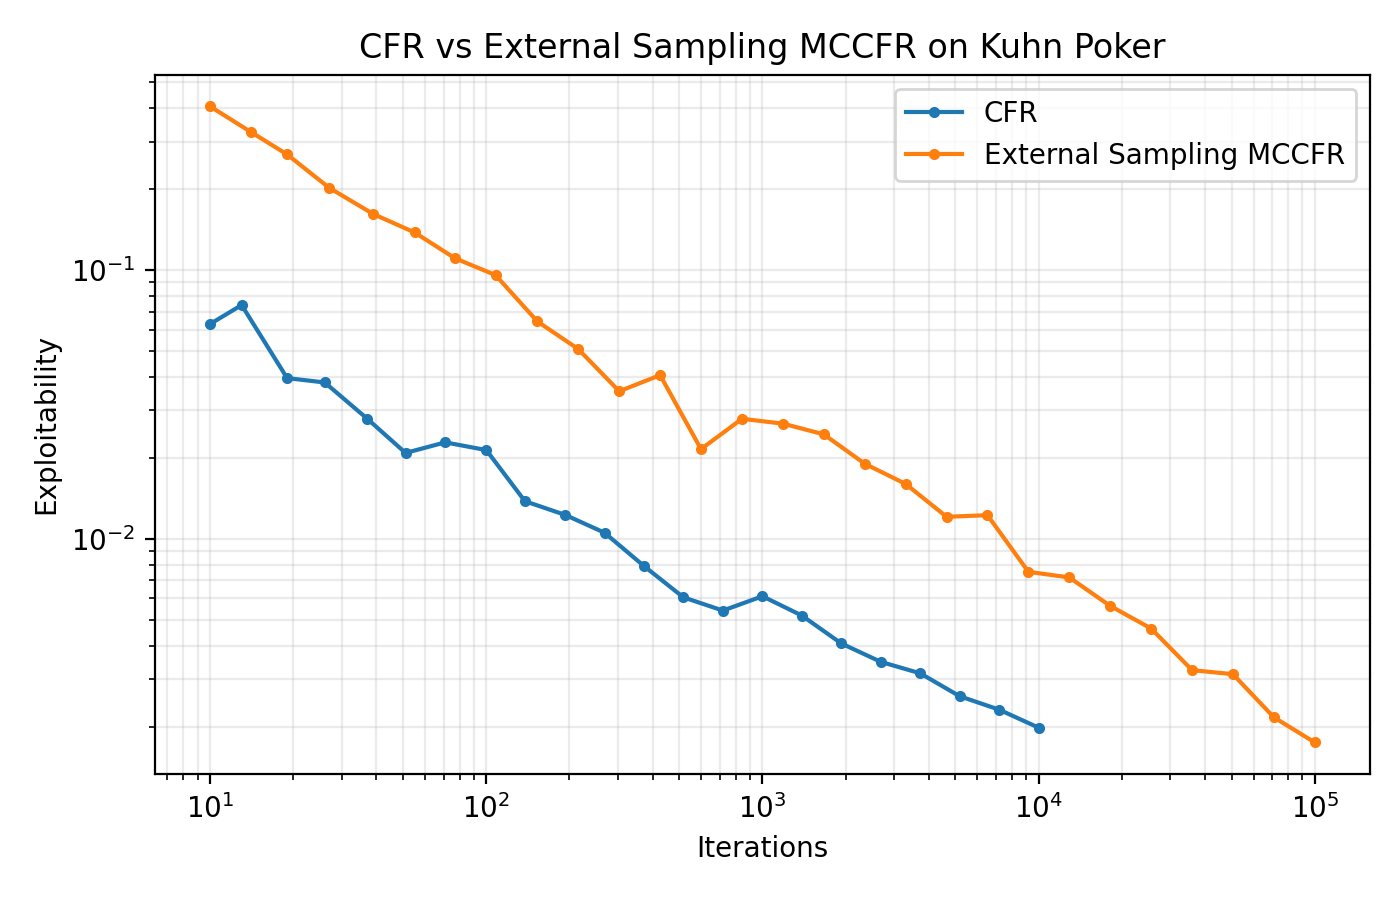
\includegraphics[width=0.82\linewidth]{figures/kuhn_cfr_vs_external_sampling_mccfr.png}
\caption{Exploitability of full-tree CFR and external-sampling MCCFR on Kuhn Poker.}
\end{figure}

\begin{figure}[H]
\centering
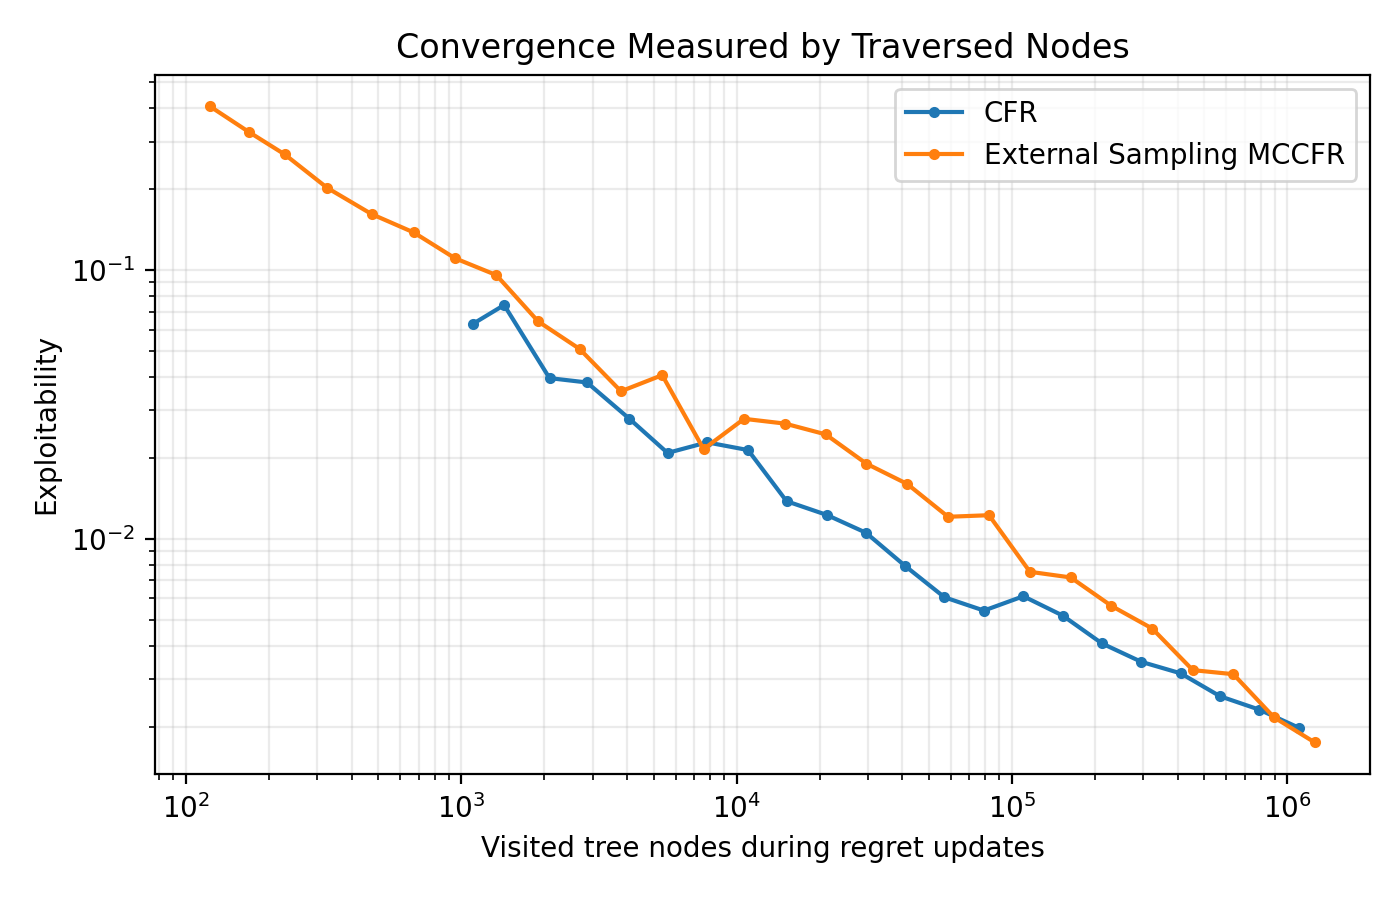
\includegraphics[width=0.82\linewidth]{figures/kuhn_mccfr_nodes.png}
\caption{The same convergence curves measured by the number of tree nodes visited during regret updates.}
\end{figure}

The learned strategies also match the qualitative structure of Kuhn Poker
equilibria. Weak hands mostly check and fold against bets, strong hands
bet or call aggressively, and the middle card mixes in response states.
This is a useful sanity check because a small exploitability number alone
does not always make implementation mistakes easy to spot.

\section{Learned Strategies}

The learned average strategies also give a qualitative sanity check. The
following table shows selected information sets from one run. The exact
numbers are not unique because Kuhn Poker has multiple equilibrium
strategies, but the broad structure is correct: weak hands usually avoid
calling, strong hands call or bet aggressively, and some bluffing appears
with the weakest card.

\begin{center}
\begin{tabular}{llrr}
\toprule
Algorithm & Information set & First action prob. & Second action prob. \\
\midrule
CFR & $J$ $(\text{check},\text{bet})$ & $0.7727$ & $0.2273$ \\
CFR & $K$ $(\text{check},\text{bet})$ & $0.2978$ & $0.7022$ \\
CFR & $Q|\text{check-bet}$ $(\text{call},\text{fold})$ & $0.5632$ & $0.4368$ \\
MCCFR & $J$ $(\text{check},\text{bet})$ & $0.7311$ & $0.2689$ \\
MCCFR & $K$ $(\text{check},\text{bet})$ & $0.2056$ & $0.7944$ \\
MCCFR & $Q|\text{check-bet}$ $(\text{call},\text{fold})$ & $0.5979$ & $0.4021$ \\
\bottomrule
\end{tabular}
\end{center}

The most useful feature of this table is not the exact decimal values,
but the pattern. With $J$, the weakest card, the strategy mixes in some
bets as bluffs but usually checks and folds when facing bets. With $K$,
the strongest card, the strategy bets frequently and calls bets almost
always. The queen is the marginal card and therefore mixes in response
states.

\section{Discussion and Bibliography}

The main lesson from this project is that MCCFR is not a different
conceptual algorithm from CFR. It is better understood as the same local
counterfactual regret update with a sampled estimator for the values.
External sampling is especially easy to understand because the update
player still branches over all actions at visited information sets.

The limitation of this project is that Kuhn Poker is small. Full-tree CFR
is already cheap, so the practical scaling advantage of MCCFR is only
visible through the node-visit counter rather than through a difficult
large-game benchmark. Natural next steps would be outcome sampling,
Leduc Poker, and abstraction methods such as bucketing.

External sampling is pedagogically attractive because it preserves the
``compare all of my actions'' step at each visited information set. This
made the implementation close to the full-tree CFR baseline. The price is
variance: a single sampled traversal sees only one chance outcome and one
opponent action at each sampled opponent decision. Outcome sampling would
go further by sampling actions for all players and using importance
weighting. That can make each iteration even cheaper, but the estimator is
usually higher variance and more delicate to implement correctly.

\sloppy

\begin{thebibliography}{9}

\bibitem{zinkevich2007}
Martin Zinkevich, Michael Johanson, Michael Bowling, and Carmelo Piccione.
\newblock Regret minimization in games with incomplete information.
\newblock In \emph{Advances in Neural Information Processing Systems 20}, 2007.
\newblock \url{https://papers.nips.cc/paper/3306-regret-minimization-in-games-with-incomplete-information}.

\bibitem{lanctot2009}
Marc Lanctot, Kevin Waugh, Martin Zinkevich, and Michael Bowling.
\newblock Monte Carlo sampling for regret minimization in extensive games.
\newblock In \emph{Advances in Neural Information Processing Systems 22}, 2009.
\newblock \url{https://papers.nips.cc/paper/3713-monte-carlo-sampling-for-regret-minimization-in-extensive-games}.

\bibitem{kuhn1950}
Harold W. Kuhn.
\newblock A simplified two-person poker.
\newblock In \emph{Contributions to the Theory of Games}, 1950.

\end{thebibliography}

\end{document}
